% !TeX spellcheck = es_ES
\documentclass[12pt, titlepage]{article}
\usepackage[letterpaper, margin=3cm]{geometry}
\usepackage[utf8]{inputenc}
\usepackage[spanish]{babel}
\usepackage{graphicx}
\usepackage{float}
\usepackage{listings}
\usepackage{color}
\usepackage{hyperref}

\definecolor{codegreen}{rgb}{0,0.6,0}
\definecolor{codegray}{rgb}{0.5,0.5,0.5}
\definecolor{codepurple}{rgb}{0.58,0,0.82}
\definecolor{backcolour}{rgb}{0.95,0.95,0.92}
 
\lstdefinestyle{mystyle}{
    backgroundcolor=\color{backcolour},   
    commentstyle=\color{codegreen},
    morekeywords={let, function},
    keywordstyle=\color{magenta},
    numberstyle=\tiny\color{codegray},
    stringstyle=\color{codepurple},
    basicstyle=\footnotesize,
    breakatwhitespace=false,         
    breaklines=true,                 
    captionpos=b,                    
    keepspaces=true,                 
    numbers=left,                    
    numbersep=5pt,                  
    showspaces=false,                
    showstringspaces=false,
    showtabs=false,                  
    tabsize=2
}
 
\lstset{style=mystyle}
%opening
\title{}
\title{Documentación del proyecto}
\author{Barrera Pérez Carlos Tonatihu \\ Profesor: Eduardo Gutiérrez Aldana \\ Administración de servicios en red \\ Grupo: 4CM2 }

\begin{document}
\maketitle
\newpage
\tableofcontents
\newpage

\section{Descripción del proyecto}
El proyecto consiste de una topología de red en la cual se presentan enrutadores, switches, servidores, gestor y clientes. Los enrutadores y servidor son monitoreados por el gestor con el objetivo de llevar un registro de los datos que estos presentan y poder detectar fallas en los equipos.

\subsection{Herramientas utilizadas}
El proyecto fue desarrollado en el ambiente de simulación \emph{GNS3} que se encuentra integrado dentro del sistema operativo \emph{Live Raizo - Linux for Virtual SysAdmin} en su versión \emph{8.17.08.30p} (\url{https://sourceforge.net/projects/live-raizo/files/}) ya que es la ultima versión que incluye \emph{Virtual Box} que se utilizo para trabajar con las maquinas virtuales que se trabaron.

Para poder trabajar de forma adecuada se adecuo una USB a modo de arranque con \emph{Raizo} y para evitar la perdida del trabajo y guardar los datos que se encuentran en \textbf{/home} y \textbf{/opt} se creo una partición en el disco duro de la computadora de trabajo. Esta partición se formateo como \textbf{ext4} y se le etiqueto como \textbf{persistence} y se le agrego un archivo llamado \textbf{persistence.conf} con la siguiente información.

\begin{lstlisting}[language=bash]
 /home
 /opt union
 /root union
\end{lstlisting}

Es importante mencionar que este método de crear persistencia se puede realizar sobre una USB y tener una USB para el boot y otra para la persistencia o ambas características en una sola USB.

En el DVD que se entregó se encuentran las carpetas \textbf{home}, \textbf{opt} con las maquinas virtuales que se trabajaron y el archivo \textbf{persistence.conf}.

De manera general otras herramientas que se utilizaron fueron \href{http://rcp100.sourceforge.net/}{RCP100} y \href{https://distro.ibiblio.org/tinycorelinux/}{TinyCore} como maquinas virtuales para los enrutadores, el gestor y el servidor.
\newpage
\section{Desarrollo}
La topología en la que se trabajo fue la siguiente.
\begin{figure}[H]
\begin{center}
 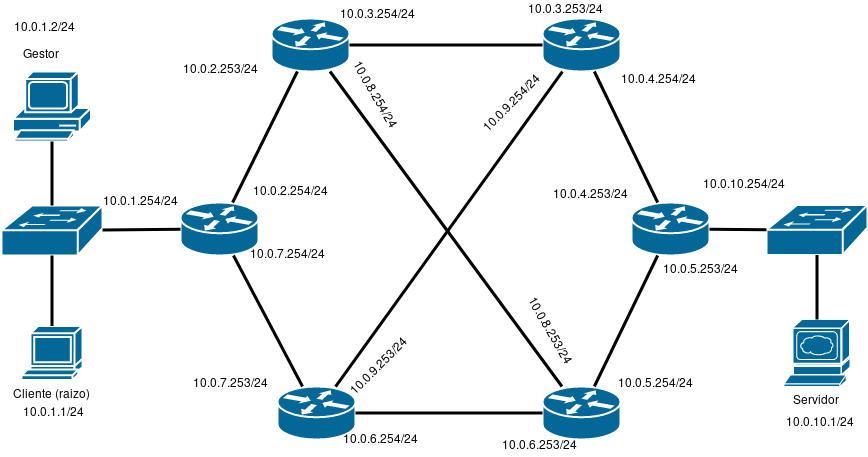
\includegraphics[width=15cm, height=8cm]{./entrega.png}
 \caption{Topología del proyecto}
 \label{fig:3318-paridad}
\end{center}
\end{figure}
La descripción de cada elemento se muestra a continuación.
\subsection{Servidor}
El servidor web fue implementado en \emph{Tiny Core} utilizando el paquete \emph{Busybox HTTPD}, el codigo que se encarga de esto se encuentra en el archivo \textbf{/opt/bootlocal.sh} para que cada vez que se encienda la computadora el servidor comience a trabajar. El código es el siguiente.

\begin{lstlisting}[language=bash]
 /usr/local/httpd/sbin/httpd -p 80 -h /home/tc/site
\end{lstlisting}
Lo que hace este código es activar el servicio de HTTP proporcionado por \emph{Busybox} en el puerto 80 indicando que la página a mostrar (index.html) se encuentra en la carpeta \textbf{/home/tc/site}.
Además, se debe de configurar una interfaz de la maquina virtual para que se pueda acceder al servidor.
\subsection{Enrutador}
Para el enrutador se utilizo RCP100, en cada uno de los enrutadores se configuraron las interfaces y el enrutamiento dinámico OSPF. Además de configurar el agente snmp necesario para llevar a cabo el monitoreo de interfaces, memoria y uso de CPU, esta configuración se realizo de la siguiente forma.
\begin{lstlisting}[language=bash]
 snmp-server contact TalesDeMileto
 snmp-server location Topolovampo
 snmp-server community soporte ro
\end{lstlisting}
\subsection{Gestor}
El gestor fue implementado en una maquina virtual con Tiny Core la cual es una distro de linux bastante liviana ya que tiene muy pocos paquetes preinstalados, por lo cual se agregaron diversos paquetes para que pueda funcionar de forma correcta, estos paquetes fueron.
\begin{itemize}
 \item net-snmp. Necesario para utilizar el protocolo de monitoreo SNMP.
 \item swaks. Es un script que permite realizar pruebas con un servidor SMTP.
 \item bc. Es un lenguaje de calculadora utilizado para realizar operaciones matemáticas en bash
 \item curl. Es una herramienta para probar diferentes protocolos, en este caso se utilizo para realizar pruebas en el servidor http.
 \item rrdtool. Es una herramienta para trabajar con bases de datos circulares, con dicha herramienta se guarda la información que se consulta y ya que es circular no crece demasiado a pesar de que se genere una gran cantidad de datos.
 \item perl. Es necesario ya que el script de swaks lo utiliza para poder funcionar. 
\end{itemize}

Todos los scripts que se utilizan para el monitoreo están elaborados en bash ya que es un lenguaje de scripting que se encuentra en muchas distribuciones de linux. Todos los scripts se ejecutan cada segundo como un demonio gracias al uso de crontab y para poder tener un control de todos los elementos que se gestionan se crea una carpeta por cada IP a monitorear y dentro de cada carpeta se crean los respectivos archivos de RRDtool para guardar datos.

El archivo de configuración de cron que se utilizo fue el siguiente.
\begin{lstlisting}[language=bash]
 #!/bin/bash
 # CRON
 * * * * * sh /home/tc/gestor/cuatro.sh
 * * * * * sh /home/tc/gestor/interfaces.sh
 * * * * * sh /home/tc/gestor/monitoreo.sh
 * * * * * sh /home/tc/gestor/ocho.sh
 * * * * * sh /home/tc/gestor/tres.sh
\end{lstlisting}

Y para lograr que cron se ejecute al encender la maquina virtual se agrega la siguiente linea de código al archivo \textbf{/opt/bootlocal.sh}.
\begin{lstlisting}[language=bash]
 crond -L /dev/null 2>&1
\end{lstlisting}

Ya que Tiny Core no guarda la carpeta donde se encuentra el archivo de configuración de cron se ejecuta el siguiente comando para que se agregue a la lista de carpetas que tienen persistencia, este paso solo se ejecuta una vez.
\begin{lstlisting}[language=bash]
 echo var/spool/cron >> /opt/.filetool.lst
\end{lstlisting}


\subsubsection{Utilización CPU}
El siguiente scripts es el encargado de determinar si se presenta una incidencia por exceso en el uso de CPU, los variables que se utilizan para cambiar su comportamiento son la lista de direcciones IP a monitorear, para el proyecto se especifico una por enrutador, el limite que se va a tolerar, la comunidad SNMP a la cual pertenece el agente, el directorio del archivo de incidencias en donde se registran los problemas que ocurren.
\begin{lstlisting}[language=bash]
 #!/bin/bash
# uno.sh
# A1 la utilizacion del CPU excede del 60%
# Lista de direcciones IP a monitorear separadas por un espacio
direcciones="10.0.1.154"
# limite a utilizar
LIMITE=60
# comunidad snmp
comunidad=public
# directorio donde se guardan los archivos que se generen
directorio=/home/tc/gestor

# Funcion de comparacion, retorna 1 si valor es mayor a limite
comparacion() {
    local me=$(awk -v lim="$1" -v valor="$2" 'BEGIN { printf (valor>lim?1:0) }')
    echo "$me"
}

for direccion in $direcciones; do
    # comando snmp y oid a consultar
    usado=$(snmpget -v 1 -c $comunidad -OQUv $direccion 1.3.6.1.2.1.25.3.3.1.2.768)

    # No debe de ser mayor que el LIMITE por ciento
    eva=$(comparacion $LIMITE $usado)

    if [ $eva -eq 1 ]; then
        # Si se excede se guarda una incidencia y se manda un correo electronico
        fecha=$(date +%y/%m/%d-%H:%M:%S)
        # Se registra la incidencia en el directorio y en el archivo incidencias
        echo "A1;$direccion;utilizacion CPU;$fecha" >> $directorio/incidencias.log
    # Codigo para enviar un correo
    #     perl swaks --to "destino@gestor.com" \
    #     --from "soporte@gestor.com" \
    #     -s 10.0.1.11:1025 \
    #     --data "Date: %DATE% \nTo: %TO_ADDRESS% \nFrom: %FROM_ADDRESS% 
    # \nSubject: A1; $direccion; utilizacion CPU 
    # \nX-Mailer: swaks v20181104 jetmore.org/john/code/swaks/
    # \n%NEW_HEADERS%\n"
    fi
done
\end{lstlisting}
La secuencia de pasos que sigue para realizar su trabajo es la siguiente.
\begin{enumerate}
 \item Realizar la consulta del OID correspondiente al uso de CPU, en este caso el 1.3.6.1.2.1.25.3.3.1.2.768.
 \item Comprarlo con la función de comparación con el limite y en el caso de que sea mayor se obtendrá un uno, cero en caso contrario.
 \item Si el resultado del paso anterior es uno se obtiene la fecha del sistema y se registra la incidencia en el archivo incidencias.log, en caso de contar con un servidor de correos se podría enviar un correo ya que se cuenta con el código necesario para hacerlo se utiliza \emph{swaks}.
\end{enumerate}

\subsubsection{Retardo en respuesta del ping}
Este script se encarga de hacer un ping a cada una de las IP que se pongan en la variable direcciones y se guarda el valor en una base de datos de RRDtool que esta configurada para llevar un registro del promedio del tiempo de respuesta a lo largo de una hora. Además, si se presenta un tiempo de respuesta mayor a 5 segundos (5000 milisegundos) se registra la incidencia en el archivo incidencias.log y en caso de contar con un servidor SMTP se podría enviar un correo electrónico.

\begin{lstlisting}[language=bash]
 #!/bin/bash
# tres.sh
# A3  Retardo en respuesta del ping mayor a 5 segundos    A3; IP; retardo en ping
# Lista de direcciones IP a monitorear separadas por un espacio
direcciones="10.0.1.254"
 # Tiempo limite en milisegundos
LIMITE=5000
# directorio donde se guardan los archivos que se generen
directorio=/home/tc/gestor

 # retorna 1 si valor es mayor que limite
comparacion() {
   local me=$(awk -v lim="$1" -v valor="$2" 'BEGIN { printf (valor>lim?1:0) }')
   echo "$me"
}

# variable=$(date +%y/%m/%d-%H:%M:%S)
for direccion in $direcciones; do
    # Si no existe se crea un subdirectorio para la ip monitorear
    subdirectorio="$directorio/$direccion"
    if [ ! -d $subdirectorio ]; then
        mkdir $subdirectorio
    fi
    base="$subdirectorio/ping.rrd"
    # Si no existe se crea la base de rrdtool del ping
    if [ ! -f $base ]; then
        rrdtool create $base  --step 60 \
        DS:tiempo:GAUGE:120:U:U \
        RRA:AVERAGE:0.5:1:60
    fi
    # Obtencion del tiempo de respuesta en ms
    tiempo=$(ping $direccion -c 1 | awk -F'time=' '/time=/ {print $2}' | awk -F' ' '{print $1}')
    #echo $tiempo
    rrdtool update $base N:$tiempo
    eva=$(comparacion $LIMITE $tiempo)

    # Se ejecuta si se supera el limite
    if [ $eva -eq 1 ]; then
        # Si se excede se guarda una incidencia y se manda un correo electronico
        fecha=$(date +%y/%m/%d-%H:%M:%S)
        # Se registra la incidencia en el directorio y en el archivo incidencias
        echo "A3;$direccion;retardo en ping;$fecha" >> $directorio/incidencias.log
    # Codigo para enviar un correo
    #     perl swaks --to "destino@gestor.com" \
    #     --from "soporte@gestor.com" \
    #     -s 10.0.1.11:1025 \
    #     --data "Date: %DATE% \nTo: %TO_ADDRESS% \nFrom: %FROM_ADDRESS% 
    # \nSubject: A3; $direccion; retardo en ping 
    # \nX-Mailer: swaks v20181104 jetmore.org/john/code/swaks/
    # \n%NEW_HEADERS%\n"
    fi
done

\end{lstlisting}


\subsubsection{Tiempo de respuesta del servidor}
El siguiente script es similar al de tiempo de respuesta del ping, solo que en este se hace la consulta al servidor HTTP y se almacena en una base de RRDtool. Se registra la incidencia en el archivo incidencias.log si es que el tiempo de respuesta es mayor a 10 segundos.
\begin{lstlisting}[language=bash]
 #!/bin/bash
# cuatro.sh
# A4 El tiempo de respuesta del servidor web excede 10 segundos
# Lista de direcciones IP a monitorear separadas por un espacio
direcciones="10.0.10.1"
 # Tiempo limite en segundos
LIMITE=10
# directorio donde se guardan los archivos que se generen
directorio=/home/tc/gestor

# Retorna 1 si valor es mayor a limite
comparacion() {
   local me=$(awk -v lim="$1" -v valor="$2" 'BEGIN { printf (valor>lim?1:0) }')
   echo "$me"
}

for direccion in $direcciones; do
    # Respuesta en segundos
    tiempo=$(curl -s -w %{time_total}\\n -o /dev/null $direccion)
    eva=$(comparacion $LIMITE $tiempo)

    #echo $tiempo

    if [ $eva -eq 1 ]; then
        # Si se excede se guarda una incidencia y se manda un correo electronico
        fecha=$(date +%y/%m/%d-%H:%M:%S)
        # Se registra la incidencia en el directorio y en el archivo incidencias
        echo "A4;$direccion;retardo http;$fecha" >> $directorio/incidencias.log
        # Envio de correo
        #    perl swaks --to "destino@gestor.com" \
        #    --from "soporte@gestor.com" \
        #    -s 10.0.1.11:1025 \
        #    --data "Date: %DATE% \nTo: %TO_ADDRESS% \nFrom: %FROM_ADDRESS% 
        #\nSubject: A4; $direccion; retardo http 
        #\nX-Mailer: swaks v20181104 jetmore.org/john/code/swaks/
        #\n%NEW_HEADERS%\n"
    fi
done

\end{lstlisting}

\subsubsection{Memoria real}
Este script revisa la memoria real de cada IP de enrutador que se encuentre en la lista de direcciones IP a monitorear y en el caso en el que la memoria disponible sea menor al 80\% se registra la incidencia. Se tienen las variables de comunidad, limite y del directorio para cambiar la funcionalidad del script de ser necesario.

Para poder obtener el porcentaje de memoria disponible se debe de obtener el valor de memoria disponible y el valor de total de memoria para a partir de estos valores calcular el porcentaje.
\begin{lstlisting}[language=bash]
 #!/bin/bash
# ocho.sh
# A8 la memoria real es menor de 80% del total
# Lista de direcciones IP a monitorerar separadas por un espacio
direcciones="10.0.1.254"
# limite a utilizar
LIMITE=0.8
# comunidad snmp
comunidad=soporte
# directorio donde se guardan los archivos que se generen
directorio=/home/tc/gestor

# Funcion de comparacion, retorna 1 si valor es menor a limite
comparacion() {
   local me=$(awk -v lim="$1" -v valor="$2" 'BEGIN { printf (valor<lim?1:0) }')
   echo "$me"
}

for direccion in $direcciones; do
    # Consulta de memoria disponible
    disponible=$(snmpget -v 1 -c $comunidad -OQUv $direccion 1.3.6.1.4.1.2021.4.6.0)
    # Consulta de memoria total
    total=$(snmpget -v 1 -c $comunidad -OQUv $direccion 1.3.6.1.4.1.2021.4.5.0)
    # Porcentaje de memoria disponible
    porcentaje=$(echo "scale=2; $disponible/$total" | bc -l)
    #echo "disponible $disponible total $total poercentaje $porcentaje"

    eva=$(comparacion $LIMITE $porcentaje)

    if [[ eva -eq 1 ]]; then
        # Si se excede se guarda una incidencia y se manda un correo electronico
        fecha=$(date +%y/%m/%d-%H:%M:%S)
        # Se registra la incidencia en el directorio y en el archivo incidencias
        echo "A8;$direccion;memoria;$fecha" >> $directorio/incidencias.log
    # Codigo para enviar un correo
    #     perl swaks --to "destino@gestor.com" \
    #     --from "soporte@gestor.com" \
    #     -s 10.0.1.11:1025 \
    #     --data "Date: %DATE% \nTo: %TO_ADDRESS% \nFrom: %FROM_ADDRESS% 
    # \nSubject: A8; $direccion; memoria 
    # \nX-Mailer: swaks v20181104 jetmore.org/john/code/swaks/
    # \n%NEW_HEADERS%\n"
    fi
done

\end{lstlisting}

\subsubsection{Monitoreo de CPU y memoria}
Este script realiza el monitoreo del CPU y la memoria para cada enrutador, guardando los datos recopilados en una base de datos de RRDtool. Al igual que en los scripts anteriores se pueden indicar varias direcciones IP a monitorear e indicar la comunidad SNMP. Este script solo guarda los datos recopilados, no realiza registro de incidencias ya que existe un script para CPU y para la memoria. 
\begin{lstlisting}[language=bash]
 #!/bin/bash
# monitoreo.sh
# script para el monitoreo de varias IP
# Lista de direcciones IP a monitorerar separadas por un espacio
direcciones="10.0.1.254"
# directorio donde se guardan los archivos que se generen
directorio=/home/tc/gestor
# comunidad snmp
comunidad=soporte

# Poner un while aqui si es necesario
for direccion in $direcciones; do
    # Si no existe se crea un subdirectorio para la ip monitorear
    subdirectorio="$directorio/$direccion"
    if [ ! -d $subdirectorio ]; then
        mkdir $subdirectorio
    fi
    base="$subdirectorio/monitoreo.rrd"
    if [ ! -f $base ]; then
        rrdtool create $base  --step 60 \
        DS:usoCPU:GAUGE:120:U:U \
        DS:usoMemoria:GAUGE:70:U:U \
        RRA:AVERAGE:0.5:1:60
    fi
    # comandos snmp y oids a consultar
    cpu_usado=$(snmpget -v 1 -c $comunidad -OQUv $direccion 1.3.6.1.2.1.25.3.3.1.2.768)
    memoria_disponible=$(snmpget -v 1 -c $comunidad -OQUv $direccion 1.3.6.1.4.1.2021.4.6.0)
    memoria_total=$(snmpget -v 1 -c $comunidad -OQUv $direccion 1.3.6.1.4.1.2021.4.5.0)
    # porcentaje de memoria usado
    porcentaje=$(echo "scale=2; (1-($memoria_disponible/$memoria_total))*100" | bc -l)
    #echo $memoria_total $memoria_disponible $porcentaje
    rrdtool update $base N:$cpu_usado:$porcentaje
done

\end{lstlisting}

Para obtener el porcentaje de memoria utilizado se obtiene la memoria disponible y la total y hacer una operación para obtener el valor a guardar en la base de datos.

\subsubsection{Monitoreo de interfaces}
Ya que cada enrutador tiene cinco interfaces diferentes se crea una base de datos para cada interfaz en la que se guardan los siguientes datos.
\begin{enumerate}
 \item ifInErrors Errores de entrada.
 \item ifInUcastpkts El numero de paquetes unicast enviados.
 \item ifInNUcastPkts EL número de paquetes no unicast enviados.
 \item ifInOctets El número total de octetos recibidos en la interfaz.
 \item ifOutOctets El número total de octetos transmitidos por la interfaz.
 \item ifSpeed Es un estimado del ancho de banda en bits por segundo.
\end{enumerate}

Esta scripts solo se encarga de guardar los datos recopilados con SNMP, no se realiza un registro de incidencias en esta parte.

\begin{lstlisting}[language=bash]
 #!/bin/bash
# interfaces.sh
# Direcciones ip a monitorear
direcciones="10.0.1.254"
# Directorio donde se guardan los archivos
directorio=/home/tc/gestor
# Comunidad snmp
comunidad=soporte
for direccion in $direcciones; do
    # num_interfaces=$(snmpwalk -v 1 -c $comunidad $direccion ifIndex | awk 'END{print NR}')
    for i in 1 2 3 4 5; do
        # Si no existe se crea un subdirectorio para la ip monitorear
        subdirectorio="$directorio/$direccion"
        if [ ! -d $subdirectorio ]; then
            mkdir $subdirectorio
        fi
        # Base de datos por interfaz
        base="$subdirectorio/interfaz-$i.rrd"
        # Si no existe se crea la base de rrdtool para cada interfaz de ip a monitorear
        if [ ! -f $base ]; then
            rrdtool create $base  --step 60 \
            DS:ifInErrors:GAUGE:120:U:U \
            DS:ifInUcastpkts:GAUGE:120:U:U \
            DS:ifInNUcastPkts:GAUGE:120:U:U \
            DS:ifInOctets:GAUGE:120:U:U \
            DS:ifOutOctets:GAUGE:120:U:U \
            DS:ifSpeed:GAUGE:120:U:U \
            RRA:AVERAGE:0.5:1:60
        fi
        ifInErrors=$(snmpget -v 1 -c $comunidad -OQUv localhost 1.3.6.1.2.1.2.2.1.14.$i)
        ifInUcastpkts=$(snmpget -v 1 -c $comunidad -OQUv localhost 1.3.6.1.2.1.2.2.1.11.$i)
        ifInNUcastPkts=$(snmpget -v 1 -c $comunidad -OQUv localhost 1.3.6.1.2.1.2.2.1.12.$i)
        ifInOctets=$(snmpget -v 1 -c $comunidad -OQUv localhost 1.3.6.1.2.1.2.2.1.10.$i)
        ifOutOctets=$(snmpget -v 1 -c $comunidad -OQUv localhost 1.3.6.1.2.1.2.2.1.16.$i)
        ifSpeed=$(snmpget -v 1 -c $comunidad -OQUv localhost 1.3.6.1.2.1.2.2.1.5.$i)
        # echo $ifInErrors $ifInUcastpkts $ifInNUcastPkts $ifInOctets $ifOutOctets $ifSpeed
        rrdtool update $base N:$ifInErrors:$ifInUcastpkts:$ifInNUcastPkts:$ifInOctets:$ifOutOctets:$ifSpeed
    done
done

\end{lstlisting}


\end{document}
